
\documentclass[journal]{IEEEtran}
\usepackage{graphicx}
\usepackage{tabularx}
\usepackage{hyperref}
\ifCLASSINFOpdf




\begin{document}

\title{About Myself and Research Interest}


\author{Sourav~Purification \\ \textit{Student, PhD in Computer Science, University of Colorado Colorado Springs}}


\maketitle


\section{Introduction}

\IEEEPARstart{I}{n} this section I am going to introduce myself as a PhD student. I shall describe my aim to achieve from this course, my research interest, as well as few things about myself.


\subsection{About myself}
I am Sourav Purification, a first year PhD student in Computer Science. I have completed my bachelor's degree in \textit{Electrical and Electronic Engineering} and worked in the various domain of telecommunication industry for the last nine years. With an aim to change my career path from an executive industry engineer to a research engineer or a research scientist I have enrolled in PhD program at UCCS. Next generation mobile network (including 5G and 6G) privacy and security will be my research focus area.

\begin{figure}[h]
    \centering
    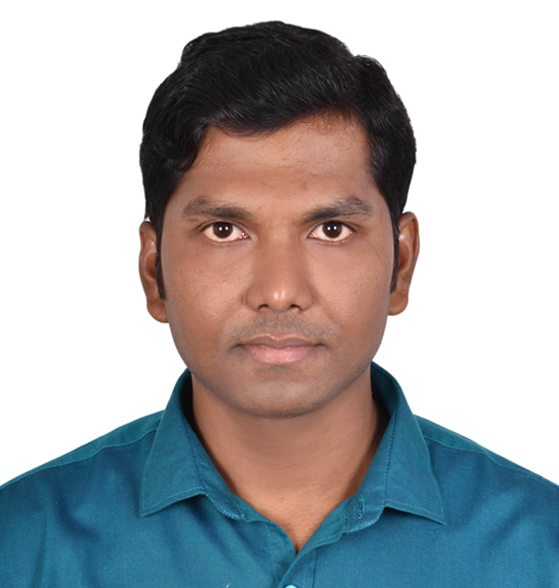
\includegraphics[width=0.4\textwidth]{Sourav.png}
\end{figure}

\subsection{Goal and Expectation}
Although, Fall 2022 is my first semester at UCCS yet I am taking CS6000: Computer Science Research course so that I can involved myself in to the research from the very beginning. I hope to learn from the course CS6000:
\begin{itemize}
    \item Research definition, outcome and different types of research
    \item Efficient way to find research papers in my domain
    \item How to read and write research papers
    \item How to grow as a researcher
\end{itemize}

\subsection{My Research Interest}
Considering my academic and professional background as well as my interest I have chosen wireless network security as my research area in a broad sense. More, specifically I want to work in mobile network security and privacy area which will include 5G and 6G networks. As communication technologies are evolving, the networks are becoming complex and more prone to security threat. User data integrity and privacy are the biggest concern for the researchers. So, I want to focus on this part. Along with mobile or cellular network I also want to work on \textit{Software Defined Networking} security, \textit{Network Function Virtualization} and related technologies. However, I am going to explore more in-depth of the domain in future. 

\section{Related Code on Github  repository}
\url{https://github.com/ocatak/6g_security} This is the github repository related to my research area. Authors are working on adversarial Machine Learning Security Problems for 6G: mmWave Beam Prediction Use-Case.

\section{Conclusion}
In this paper I have discussed my research interest and included a Git Repo related to my area of interest. Your are open to ask questions in Next Section.


\section{Questions}
\\
\textbf{Question 1}

Hi Sourav,

I like the adversarial attack that you mentioned since I will also be focusing on Machine Learning. Are you focusing only on 6G or you will include 5G?


%Ask your question here
Can you please elaborate on network function virtualization? Thanks.

\\
\textbf{Answer 1:}


\\
\textbf{Question 2}

%Ask your question here

\\
\textbf{Answer 2:}


\end{document}


